% =====================================================================
%  monoT5 Per-Head Activation Patching + Ablation — Full Experiment Report
%  Compile with:  pdflatex head_patching_experiment_report.tex  (run twice)
%  Figure paths are relative to this file (outputs/...), so compile
%  from the 03_monot5_head_patching_ablation/ directory.
% =====================================================================
\documentclass[11pt]{article}

\usepackage[margin=1in]{geometry}
\usepackage{amsmath, amssymb}
\usepackage{graphicx}
\usepackage{booktabs}
\usepackage{longtable}
\usepackage{array}
\usepackage{float}
\usepackage{xcolor}
\usepackage{caption}
\usepackage{subcaption}
\usepackage{enumitem}
\usepackage{listings}
\usepackage[hidelinks]{hyperref}

\definecolor{codegray}{gray}{0.95}
\lstset{
  basicstyle=\ttfamily\footnotesize,
  backgroundcolor=\color{codegray},
  breaklines=true,
  frame=single,
  columns=fullflexible,
  keepspaces=true,
}

\newcommand{\fwd}{\ensuremath{e^{\mathrm{fwd}}}}
\newcommand{\rev}{\ensuremath{e^{\mathrm{rev}}}}
\newcommand{\score}{\operatorname{score}}
\newcommand{\comb}{\ensuremath{e^{\mathrm{comb}}}}

\title{\textbf{Per-Head Activation Patching and Ablation of the monoT5 \\[2pt]
Decoder under Keyword-Stuffing Adversarial Attacks} \\[6pt]
\large A Head-Level Refinement of the Layer-Level Causal-Tracing Study}
\author{Information-Retrieval Adversarial-Evaluation Project}
\date{\today}

\begin{document}
\maketitle

\begin{abstract}
This report documents an \emph{attention-head-level} activation-patching and
ablation experiment on \texttt{castorini/monot5-base-msmarco}, extending the
layer-level causal-tracing study (Experiment~1) down to individual attention
heads. Experiment~1 found that the injected ``relevance'' signal of a
keyword-stuffing attack is concentrated in the \emph{decoder cross-attention}
of the final layers, but a whole sub-layer contains 12 heads acting in
parallel and the layer-level method cannot say which of them carry the
signal. Here we intervene directly on the 288 individual decoder attention
heads (12 layers $\times$ \{self-attention, cross-attention\} $\times$ 12
heads), computing forward/reverse patching and zero/mean ablation for each
head, across a breadth sweep of 105 attacks and a depth sweep of 100 examples
on the canonical attack. Both sweeps run at \textbf{100 examples per attack}
(Grid~A was originally piloted at 10/attack; Section~\ref{sec:n100}
documents what the ten-fold increase in sample size changed). The signal is
sparse: \textbf{33 of 288 heads} (11.5\%) show a mean combined effect
exceeding 0.02, and \textbf{31 of those 33 are cross-attention heads}. The
single most important head, \textbf{decoder layer 11, cross-attention,
head~3}, is positive on \textbf{104 of the 105 attacks} (range
$-0.096$ to $0.721$, negative only on \texttt{bar\_random\_4}), making it a
near-universal carrier of the attack signal, while \textbf{layer 9,
cross-attention, head~2} attains one of the single highest effects of any
head on any attack ($0.293$ on \texttt{true\_end\_4}) but is inert
($<0.01$) on 25 of 105 attacks and mildly negative on others — an
attack-specific rather than universal head. A methodological finding of
independent interest: \emph{zero} ablation of the top heads produces large
score changes that are almost identical on clean and attacked inputs (a
generic, non-attack-specific disruption), whereas \emph{mean} ablation
(replacing the head's output with its padded-control activation) produces a
much smaller but genuinely attack-specific score drop. Mean ablation is
therefore the more trustworthy diagnostic of the two for isolating
attack-specific head function. A further revision at $n=100$: the
correlation between the breadth (Grid~A) and depth (Grid~B) sweeps, initially
$r=0.84$ at $n=10$, drops to $r=0.42$ once both have equal statistical
power — attack-specificity turns out to be more pervasive than the pilot
sample suggested, and only 7 of the 33 breadth-flagged heads are also
significant for the single canonical attack.
\end{abstract}

\tableofcontents
\newpage

% =====================================================================
\section{Introduction and Motivation}
% =====================================================================

Experiment~1 (layer-level activation patching, see
\texttt{01\_monot5\_layer\_patching/patching\_experiment\_report.tex}) showed
that a keyword-stuffing attack against monoT5 is not carried by one early
component but accumulates with depth, becoming a decision in the top few
layers, concentrated in decoder cross-attention. That analysis patches or
reads out whole sub-layer outputs, i.e.\ the concatenated contribution of all
12 attention heads at once. This leaves a mechanistic question unanswered:

\begin{quote}
\itshape Within a cross-attention sub-layer that has been identified as
important, is the signal spread evenly across its 12 heads, or is it carried
by one or two specific heads while the rest are along for the ride?
\end{quote}

Answering this matters both for interpretability (a single head is a much
sharper, more falsifiable causal claim than ``a sub-layer'') and for defence
(surgically ablating one head is a far less invasive intervention than
disabling an entire cross-attention block). This experiment repeats the
forward/reverse patching methodology of Experiment~1, and adds a
complementary \emph{ablation} methodology (zero and mean), at the
granularity of individual attention heads, restricted to the decoder (where
Experiment~1 found the strongest and most consistent late-layer signal).

% =====================================================================
\section{Background}
% =====================================================================

\subsection{Where a ``head'' lives in T5 attention}

T5 multi-head attention computes, for each of its 12 heads $h$, a per-head
output of dimension $d_{kv}=64$, concatenates them, and projects the
concatenation back to model space with a single linear map $W_o$ (no bias):
\begin{equation}
\text{out} \;=\; W_o \cdot \operatorname{concat}\big(\text{head}_0,\dots,\text{head}_{11}\big),
\qquad \text{head}_h \in \mathbb{R}^{d_{kv}},\ \ d_{kv}=64,\ \ 12\times64=d_{\text{model}}=768.
\label{eq:headconcat}
\end{equation}
Because $W_o$ has \emph{no bias}, replacing or zeroing the contiguous slice
$[\,h\cdot d_{kv} : (h{+}1)\cdot d_{kv}\,]$ of the concatenated vector that
feeds $W_o$ replaces or zeroes \emph{exactly} that head's additive
contribution to the residual stream — nothing else changes. We therefore
intervene with PyTorch forward \emph{pre}-hooks registered on each
attention's \texttt{.o} projection module, immediately before $W_o$ is
applied (\texttt{headlib/head\_hooks.py}).

\subsection{Scope: decoder-only, two components, 288 head-slots}

monoT5-base has 12 decoder layers, each with a self-attention sub-layer and a
cross-attention sub-layer (the decoder feed-forward has no heads and is
excluded). The scope is therefore
\[
12~\text{layers} \times 2~\text{components} \times 12~\text{heads}
\;=\; 288~\text{head-slots.}
\]
The encoder is out of scope here; Experiment~1 already covers encoder
components at layer granularity.

\subsection{Why a single decoder step makes this tractable}

monoT5 scoring performs exactly one decoder step (Eq.~\ref{eq:score} below),
so every decoder attention module's \texttt{.o}-input has query length~1:
shape $(1,1,768)$, \emph{regardless of the encoder input length}. Control,
attack, and clean-input runs are therefore always shape-compatible at the
point of intervention — token alignment (Experiment~1's
\texttt{src/alignment.py}) is only needed to build the padded-control
\emph{encoder} input, not for the head-level patch itself.

\subsection{Scoring (unchanged from Experiment 1)}

\begin{equation}
\score \;=\; \operatorname{logit}(\texttt{true}) - \operatorname{logit}(\texttt{false})
\label{eq:score}
\end{equation}
read out at the single decoder step, exactly as in Experiment~1
(Eq.~1 of that report).

% =====================================================================
\section{Experimental Setup}
% =====================================================================

\subsection{Configuration}

\begin{table}[H]
\centering
\caption{Experiment configuration (\texttt{configs/default.yaml}).}
\label{tab:config}
\begin{tabular}{ll}
\toprule
Parameter & Value \\
\midrule
Model checkpoint            & \texttt{castorini/monot5-base-msmarco} \\
Decoder layers $\times$ components $\times$ heads
                             & $12 \times 2 \times 12 = 288$ head-slots \\
Heads per attention / head dim $d_{kv}$ & 12 / 64 \\
Max encoder length           & 512 tokens \\
Device                       & GPU (SLURM, 1$\times$ L40) \\
\midrule
Attack grid                  & inherited from Experiment~1's
                               \texttt{configs/multi\_attack.yaml}
                               (7 tokens $\times$ 3 positions $\times$
                               5 reps $=105$ attacks) \\
Canonical attack (Grid~B)    & \texttt{relevant\_start\_5} \\
Ablation methods             & zero, mean \\
Example reuse                & Experiment~1's
                               \texttt{selected\_examples.jsonl}
                               (top-$n$ by attack\_delta\_vs\_control) \\
Random seed                  & 42 \\
\bottomrule
\end{tabular}
\end{table}

\subsection{The four runs}

\begin{table}[H]
\centering
\caption{The four runs and what each computes.}
\label{tab:runs}
\begin{tabular}{lllll}
\toprule
Run & Attacks & Examples & Base input & Metrics \\
\midrule
Grid~A & all 105       & 100/attack (capped by availability, min 80)  & attack  & fwd, rev, comb, zero, mean \\
Grid~B & \texttt{relevant\_start\_5} & 100 & attack & fwd, rev, comb, zero, mean \\
Clean~A & 105 (matched clean) & 100/attack & clean & zero, mean (side-effect check) \\
Clean~B & \texttt{relevant\_start\_5} (matched clean) & 100 & clean & zero, mean (side-effect check) \\
\bottomrule
\end{tabular}
\end{table}

Grid~A trades depth for breadth (does a head matter for \emph{most} attacks?);
Grid~B trades breadth for depth (a stable estimate for \emph{one} attack, and
a sanity check against Grid~A). Clean~A/B measure whether ablating a head
also disturbs \emph{ordinary}, unattacked scoring — the side-effect check
that separates a safe, attack-specific ablation target from a risky one that
breaks normal ranking.

\paragraph{Revision note.} Grid~A and Clean~A were originally run at
10~examples/attack (1{,}050 total) and have since been re-run at
100~examples/attack (10{,}432 total, capped by availability — 7 of the 105
attacks have fewer than 100 selected examples) to match Grid~B/Clean~B's
depth. All numbers, tables, and figures in this report reflect the
100-example run; Section~\ref{sec:n100} discusses specifically what changed
between the two sample sizes, since two of the original report's claims
(head universality and Grid~A/B agreement) do not hold up as cleanly with
ten times the statistical power.

\subsection{Example reuse}

Rather than re-scoring and re-selecting examples, all four runs load
Experiment~1's per-attack \texttt{selected\_examples.jsonl}
(query, passage, attacked passage, and all three scores), sorted by
\texttt{attack\_delta\_vs\_control} descending, and take the top $n$. This
guarantees the head-level results are computed on exactly the examples that
Experiment~1's layer-level results were computed on, making the two reports
directly comparable. (A from-scratch scoring fallback exists for attacks
without a saved selection, but was not exercised: all 105 attacks in this
run had a valid selection file with 80--200 examples each.)

% =====================================================================
\section{Methodology: Per-Head Patching and Ablation Metrics}
% =====================================================================

\subsection{Forward / reverse / combined patching (per head)}

Identical in form to Experiment~1's Eqs.~4--6, but applied to a single head's
slice of the \texttt{.o}-input rather than a whole sub-layer's residual
contribution. With $\Delta=\score_{\text{attack}}-\score_{\text{control}}$:
\begin{align}
\fwd_{L,C,h} &= \frac{\score_{\text{patched-fwd}} - \score_{\text{control}}}{\Delta}
&&\text{(control base, head $h$ set to its attack activation)} \label{eq:hfwd}\\
\rev_{L,C,h} &= \frac{\score_{\text{attack}} - \score_{\text{patched-rev}}}{\Delta}
&&\text{(attack base, head $h$ set to its control activation)} \label{eq:hrev}\\
\comb_{L,C,h} &= \min(\fwd_{L,C,h}, \rev_{L,C,h}) \label{eq:hcomb}
\end{align}
Examples with $|\Delta|<10^{-4}$ are skipped (identical
\texttt{SKIP\_EPSILON} guard as Experiment~1).

\subsection{Zero and mean ablation}

\begin{description}[leftmargin=2em,style=nextline]
  \item[Zero ablation.] Head $h$'s slice of the \texttt{.o}-input is set to
  the zero vector — the head contributes nothing to the residual stream.
  \item[Mean ablation.] Head $h$'s slice is replaced with the corresponding
  slice from the \emph{padded-control} (Type~B) run — a plausible,
  distribution-matched substitute rather than an out-of-distribution zero.
\end{description}
Both are computed on the \textbf{attack} input for Grid~A/B and on the
\textbf{clean} input for Clean~A/B:
\begin{equation}
\text{score\_drop}_{\text{zero/mean}} \;=\; \score_{\text{before}} - \score_{\text{ablated-zero/mean}},
\qquad
\score_{\text{before}} = \begin{cases}\score_{\text{attack}} & \text{Grid A/B}\\ \score_{\text{clean}} & \text{Clean A/B}\end{cases}
\label{eq:drop}
\end{equation}

\paragraph{An algebraic identity worth stating explicitly.} On the
\emph{attack} base, mean ablation (attack run, head replaced by its control
activation) and reverse patching (Eq.~\ref{eq:hrev}) are the \emph{same
computation}. The pipeline computes it once per head and writes it to both
\texttt{score\_ablated\_mean} and \texttt{score\_patched\_rev}; they are
identical by construction in Grid~A/B, and this was verified in unit tests
(\texttt{tests/test\_head\_engine.py}). The two columns diverge only on
Clean~A/B, where mean ablation is a genuinely distinct computation (clean
run, head replaced by control activation).

\subsection{Batched-over-heads scoring (an exactness-preserving speedup)}

Because all 12 heads of one (layer, component) slot can be patched
independently, all 12 are scored in a \emph{single} decoder pass: a batch of
12 identical input rows, where row $h$ has \emph{only} head $h$'s slice
replaced (a block-diagonal mask, \texttt{headlib/head\_hooks.py}). A second
exact speedup reuses the encoder's hidden states across every patched
decoder pass of the same input, since every intervention is decoder-side.
Both speedups are verified exact against a one-head-at-a-time reference and
against Experiment~1's layer-level patch (replacing all 12 head slices at
once reproduces the layer-level contribution patch bit-for-bit) in
\texttt{tests/test\_head\_engine.py} (13/13 passing).

% =====================================================================
\section{The Pipeline}
% =====================================================================

\begin{description}[leftmargin=1.8em,style=nextline]
  \item[\texttt{headlib/head\_hooks.py}] Per-head pre-hooks on each
    attention's \texttt{.o} projection: cache hook, block-diagonal
    per-row patch/ablate hook, and a full-slice replace hook (used only by
    the cross-experiment consistency test).
  \item[\texttt{headlib/engine.py}] The scoring engine: encoder-state reuse,
    batched-over-heads decoder passes, and the per-example drivers
    \texttt{run\_grid\_example} (Grid~A/B) and \texttt{run\_clean\_example}
    (Clean~A/B).
  \item[\texttt{headlib/run\_utils.py}] Config loading (with
    \texttt{attacks.inherit\_from} pulling in Experiment~1's 105-attack
    grid) and example reuse/fallback selection.
  \item[\texttt{scripts/01\_run\_head\_grid.py}] Driver for all four runs;
    resume-safe per (run, attack) via \texttt{status.json}, writing one
    \texttt{head\_results.csv} per attack per run.
  \item[\texttt{scripts/02\_aggregate.py}] Derived mean$\pm$std summaries per
    (head, attack) and per head, from the per-example CSVs.
  \item[\texttt{scripts/03\_make\_plots.py}] The five figures presented in
    Section~\ref{sec:results}.
\end{description}
One upstream change was made to Experiment~1's code to support this
experiment: \texttt{score\_pairs\_general()} was added to
\texttt{01\_monot5\_layer\_patching/src/scoring.py}, factoring out the
general-alignment scoring loop that was previously embedded in Experiment~1's
script~10, so it could be imported rather than duplicated. No other
Experiment~1 files were modified.

% =====================================================================
\section{Output Files}
% =====================================================================

\begin{longtable}{p{0.46\textwidth}p{0.48\textwidth}}
\toprule
File & Contents \\
\midrule
\endhead
\texttt{outputs/\{run\}/attacks/\{attack\}/head\_results.csv} &
  \textbf{Primary data.} One row per (head, example): all scores, both
  patching effects, both ablation drops. Never aggregated in place. \\
\texttt{outputs/\{run\}/attacks/\{attack\}/selected\_examples.jsonl} &
  The exact examples used (reused from Experiment~1 or freshly selected). \\
\texttt{outputs/\{run\}/attacks/\{attack\}/status.json} &
  Resume bookkeeping: success/failure, counts, error trace if any. \\
\texttt{outputs/\{run\}/aggregated/head\_attack\_summary.csv} &
  Derived: mean$\pm$std$\pm n$ per (head, attack). \\
\texttt{outputs/\{run\}/aggregated/head\_summary.csv} &
  Derived: mean$\pm$std$\pm n$ per head, pooled over attacks and examples. \\
\bottomrule
\end{longtable}

% =====================================================================
\section{Results}
\label{sec:results}
% =====================================================================

The run executed on 1$\times$ L40 GPU in $\approx$4 hours wall-clock,
processing all $105+1+105+1=212$ (run, attack) units with
\textbf{zero failures and zero token-alignment failures}, writing
6{,}066{,}744 per-example rows (grid\_a: 3{,}004{,}416; grid\_b: 28{,}800;
clean\_a: 3{,}004{,}416; clean\_b: 28{,}800) totalling 1.5~GB.

\subsection{Localisation: which heads carry the signal}

\begin{figure}[H]
  \centering
  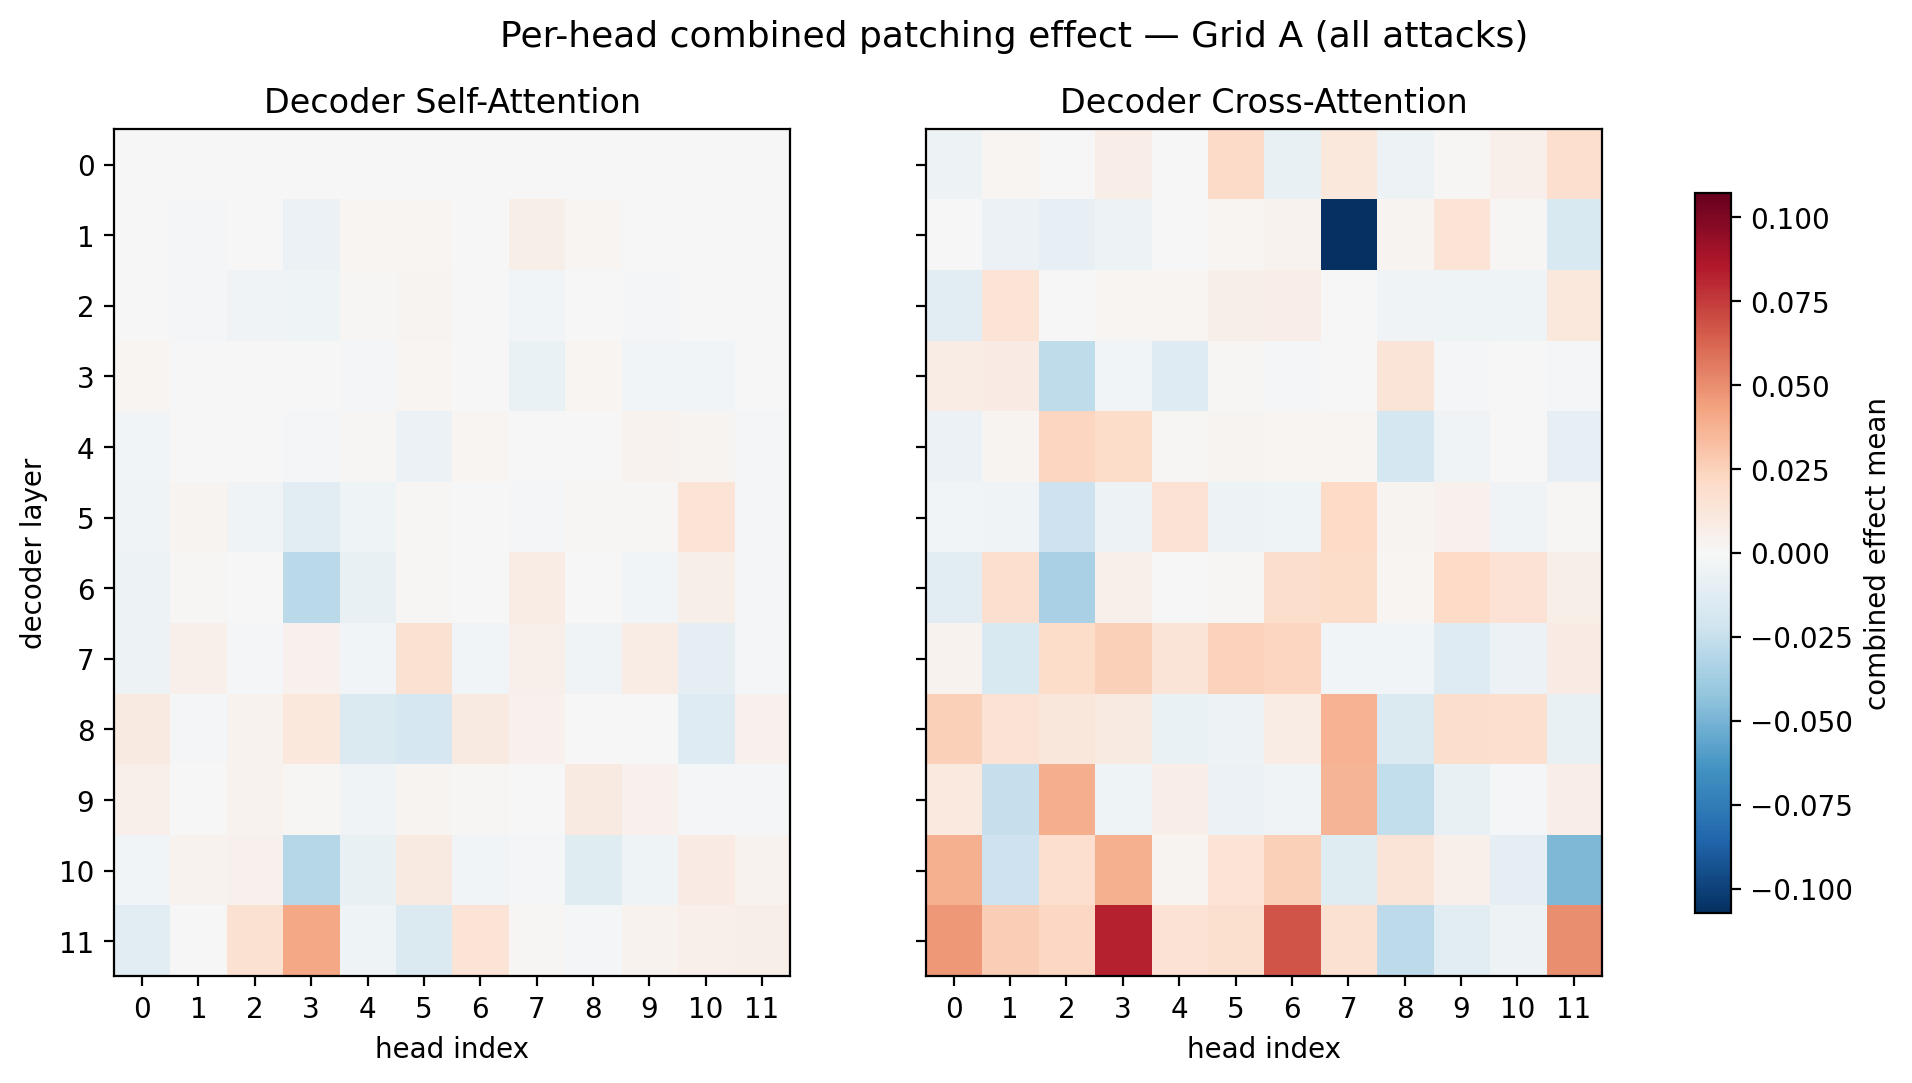
\includegraphics[width=0.95\textwidth]{outputs/plots/head_heatmap_grid_a.png}
  \caption{Mean combined effect $\comb_{L,C,h}$ per head, Grid~A (all 105
  attacks, $n=100$ each). Rows are decoder layers, columns are heads,
  separate panels for self- and cross-attention. Signal is essentially
  absent from self-attention and concentrated in a handful of late-layer
  cross-attention cells.}
  \label{fig:heatmap_a}
\end{figure}

\begin{table}[H]
\centering
\caption{Top 10 heads by mean combined effect, Grid~A (105 attacks, $n=100$).}
\label{tab:top8}
\begin{tabular}{lrrrrr}
\toprule
Head & $\comb$ & $\fwd$ & $\rev$ & drop$_{\text{zero}}$ & drop$_{\text{mean}}$ \\
\midrule
L11-X-H3  & 0.0822 & 0.0833 & 0.0837 & $-$0.437 & 0.015 \\
L11-X-H6  & 0.0677 & 0.0682 & 0.0691 & $-$0.193 & 0.009 \\
L11-X-H11 & 0.0500 & 0.0505 & 0.0512 & $-$0.325 & 0.012 \\
L11-X-H0  & 0.0466 & 0.0469 & 0.0478 & $-$0.123 & 0.008 \\
L11-S-H3  & 0.0416 & 0.0430 & 0.0420 & \phantom{$-$}0.000 & 0.001 \\
L9-X-H2   & 0.0391 & 0.0414 & 0.0424 & $-$0.155 & 0.011 \\
L10-X-H0  & 0.0384 & 0.0425 & 0.0415 & \phantom{$-$}0.331 & 0.003 \\
L10-X-H3  & 0.0378 & 0.0385 & 0.0400 & $-$0.030 & 0.004 \\
L8-X-H7   & 0.0373 & 0.0416 & 0.0399 & $-$0.173 & 0.013 \\
L9-X-H7   & 0.0365 & 0.0379 & 0.0387 & $-$0.084 & 0.005 \\
\bottomrule
\end{tabular}
\\[4pt]
\footnotesize X = cross-attention, S = self-attention. 9 of the top 10 are
cross-attention; \texttt{L11-S-H3} is the sole self-attention head to break
into the top 10 at this sample size (it did not appear in the $n=10$ top 8).
\end{table}

\paragraph{Sparsity.} At $n=100$, \textbf{33 of the 288 head-slots} (11.5\%)
exceed a mean combined effect of $0.02$ — more than double the 13 found at
$n=10$ (Section~\ref{sec:n100} discusses why). 31 of the 33 are
cross-attention; the two self-attention exceptions are \texttt{L11-S-H3}
($0.042$) and \texttt{L10-S-H3} ($0.021$, barely over threshold). The most
negative head is now \texttt{L1-X-H7} ($-0.107$), driven by one extreme
outlier attack (\texttt{bar\_random\_4}) rather than a genuine
counter-mechanism — its \emph{median} across attacks is only $-0.012$; see
Section~\ref{sec:n100} for why mean and median disagree so sharply here.
Overall mean combined effect is $0.0040$ for cross-attention versus
$-0.00002$ for self-attention (self-attention is now indistinguishable from
zero on average, an even starker separation than at $n=10$), and
cross-attention's layer-wise mean is highest at layer~11 ($0.0249$), though
no longer strictly monotonic with depth (layer~1 is slightly negative,
$-0.0100$).

\paragraph{Forward and reverse agree almost exactly.} Across all 288 heads,
the mean $|\fwd - \rev|$ is $0.00034$ — every head that is sufficient to
carry the attack (high $\fwd$) is, to a very close approximation, equally
necessary (equally high $\rev$). The mechanism is ``clean'': there is no
head that is sufficient but not necessary, or vice versa, among the
important heads. This holds identically at both sample sizes.

\subsection{Depth sanity check: Grid B}

\begin{figure}[H]
  \centering
  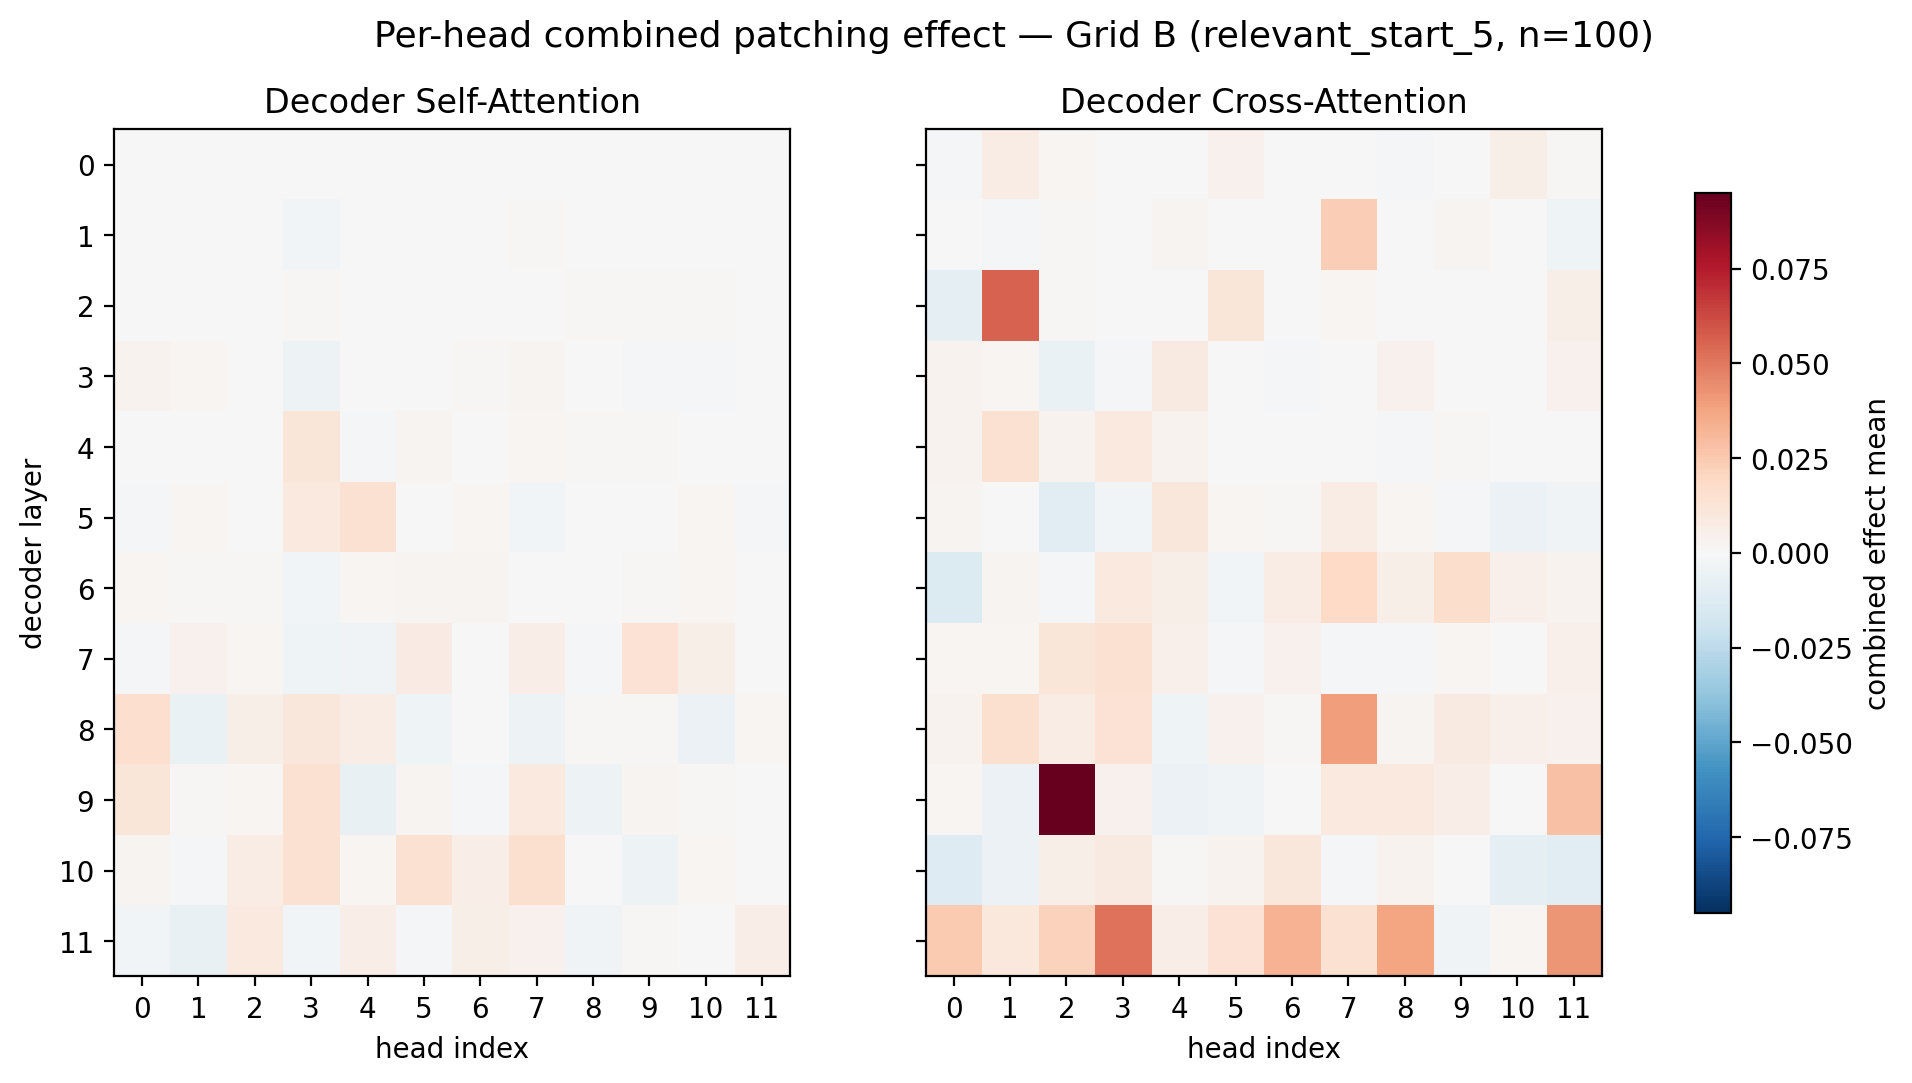
\includegraphics[width=0.95\textwidth]{outputs/plots/head_heatmap_grid_b.png}
  \caption{Same layout as Fig.~\ref{fig:heatmap_a}, for Grid~B (single
  canonical attack \texttt{relevant\_start\_5}, $n=100$ examples,
  unchanged between the two Grid~A sample sizes).}
  \label{fig:heatmap_b}
\end{figure}

Grid~B's top head for this one attack is \texttt{L9-X-H2} ($\comb=0.095$,
more than double its Grid~A value across all attacks, since this head is
more attack-specific — see below), followed by \texttt{L2-X-H1} (0.056),
\texttt{L11-X-H3} (0.052), \texttt{L11-X-H11} (0.042) and \texttt{L8-X-H7}
(0.040). \textbf{At $n=100$ for both grids, the Pearson correlation between
Grid~A's and Grid~B's per-head mean combined effect drops to $r=0.42$
(Spearman $\rho=0.45$)} — substantially weaker than the $r=0.84$ observed
when Grid~A was still at $n=10$. Only \textbf{7 of the 33} heads that clear
the $0.02$ threshold in Grid~A also clear it in Grid~B
(\texttt{L8-X-H7}, \texttt{L9-X-H2}, \texttt{L11-X-H0}, \texttt{L11-X-H2},
\texttt{L11-X-H3}, \texttt{L11-X-H6}, \texttt{L11-X-H11}). See
Section~\ref{sec:n100} for why this is a genuine finding about
attack-specificity, not a regression in data quality.

\subsection{Universal vs. attack-specific heads}

\begin{figure}[H]
  \centering
  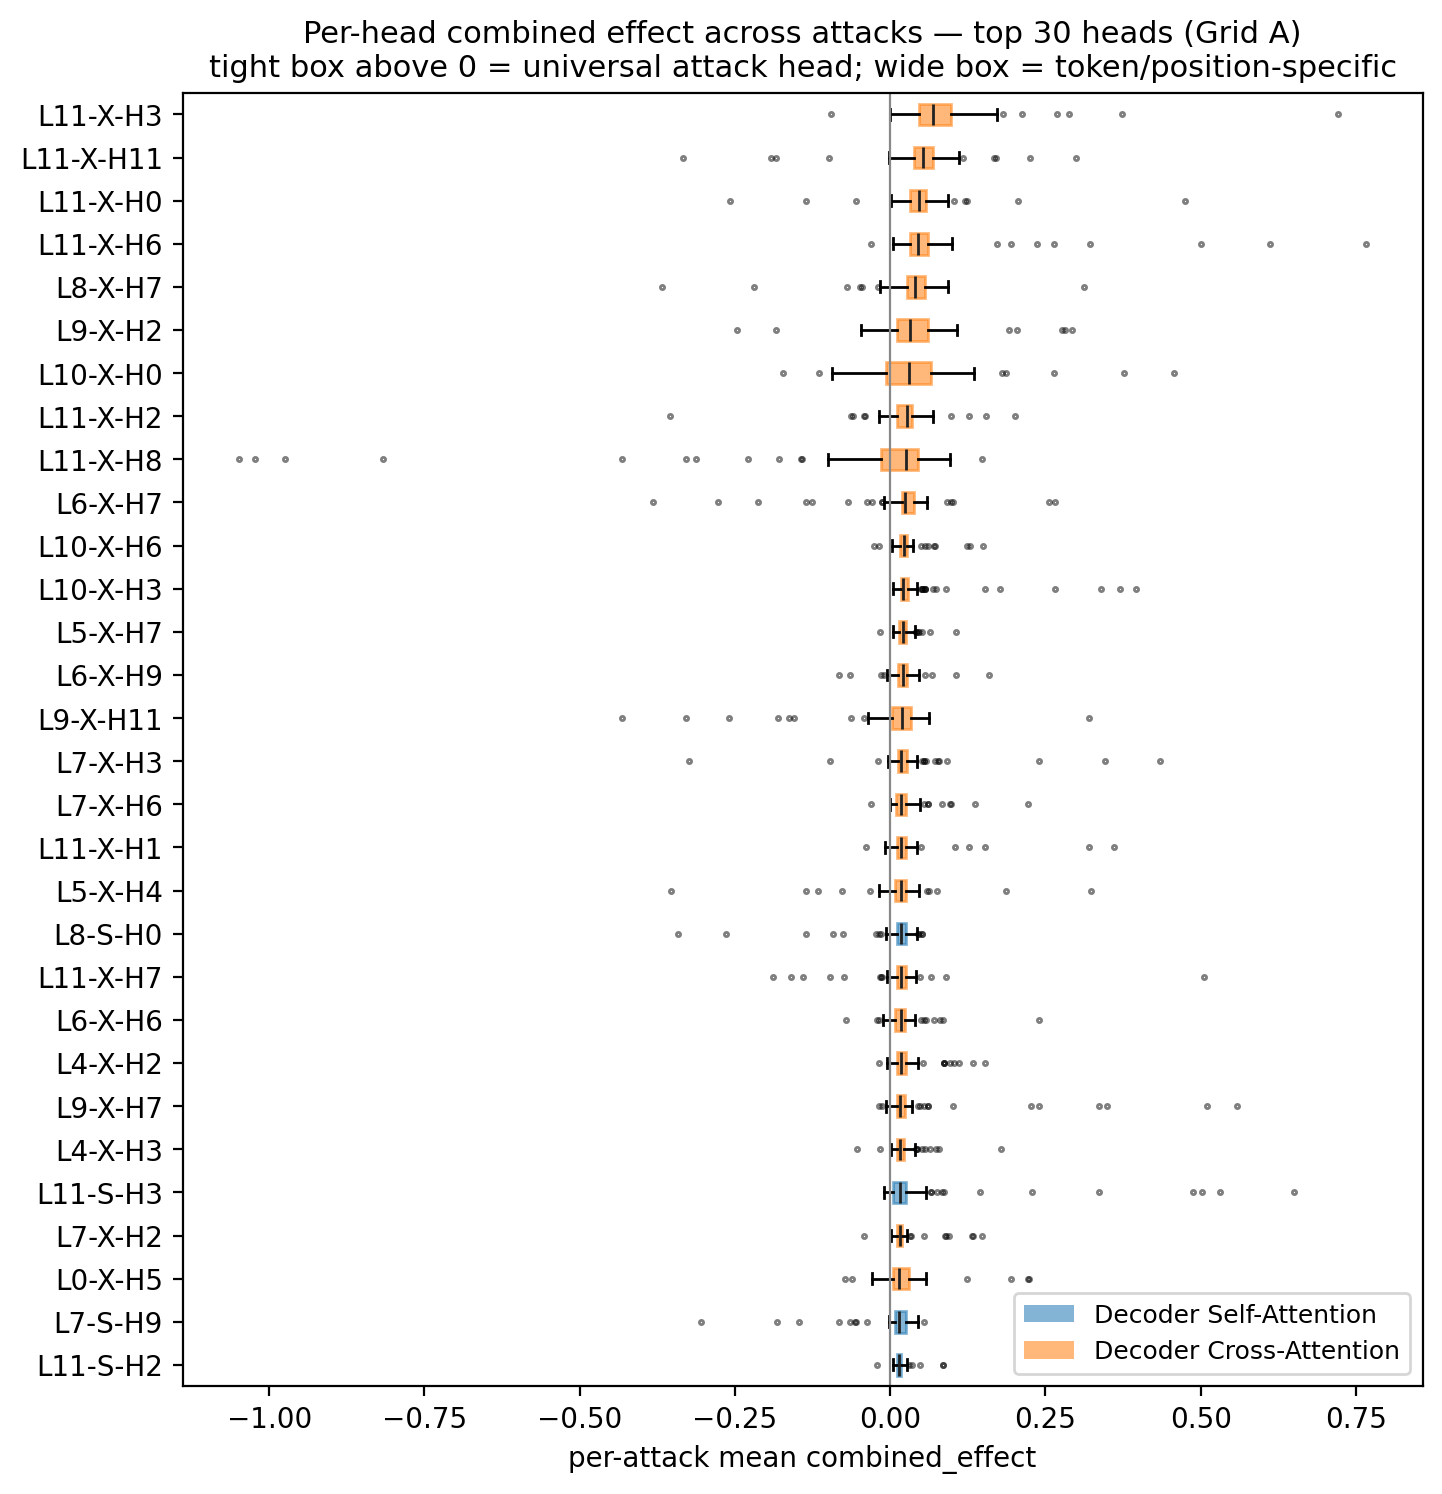
\includegraphics[width=0.95\textwidth]{outputs/plots/per_head_effect_across_attacks.png}
  \caption{Distribution of per-attack mean combined effect across the 105
  attacks, for the top 30 heads (Grid~A, $n=100$). A tight box well above
  zero indicates a head that helps on nearly every attack; a wide box or
  heavy outliers indicate a head that helps enormously on a few attacks but
  is inert or harmful on others.}
  \label{fig:boxplot}
\end{figure}

The two headline heads still illustrate opposite ends of this spectrum, but
with more nuance than the $n=10$ estimate suggested:
\begin{itemize}[nosep]
  \item \textbf{\texttt{L11-X-H3} is near-universal, not literally
  universal.} Its combined effect is positive on \textbf{104 of 105 attacks}
  (median $0.069$, range $[-0.096,\,0.721]$) — negative only on
  \texttt{bar\_random\_4} ($-0.096$), and below $0.01$ on one further attack.
  The maximum ($0.721$ on \texttt{true\_end\_3}) is far above the $n=10$
  estimate's reported ceiling of $0.102$, and the standard deviation across
  attacks ($0.085$) is five times the $n=10$ estimate ($0.017$) — the small
  sample understated both the head's peak effect and its true variability.
  \item \textbf{\texttt{L9-X-H2} is attack-specific.} Its distribution
  remains wide (median $0.031$), consistent with the $n=10$ finding that it
  keys on specific tokens or positions rather than carrying a token-agnostic
  notion of ``stuffed keywords''.
\end{itemize}

\subsection{A methodological caveat: zero ablation is not attack-specific}

\begin{figure}[H]
  \centering
  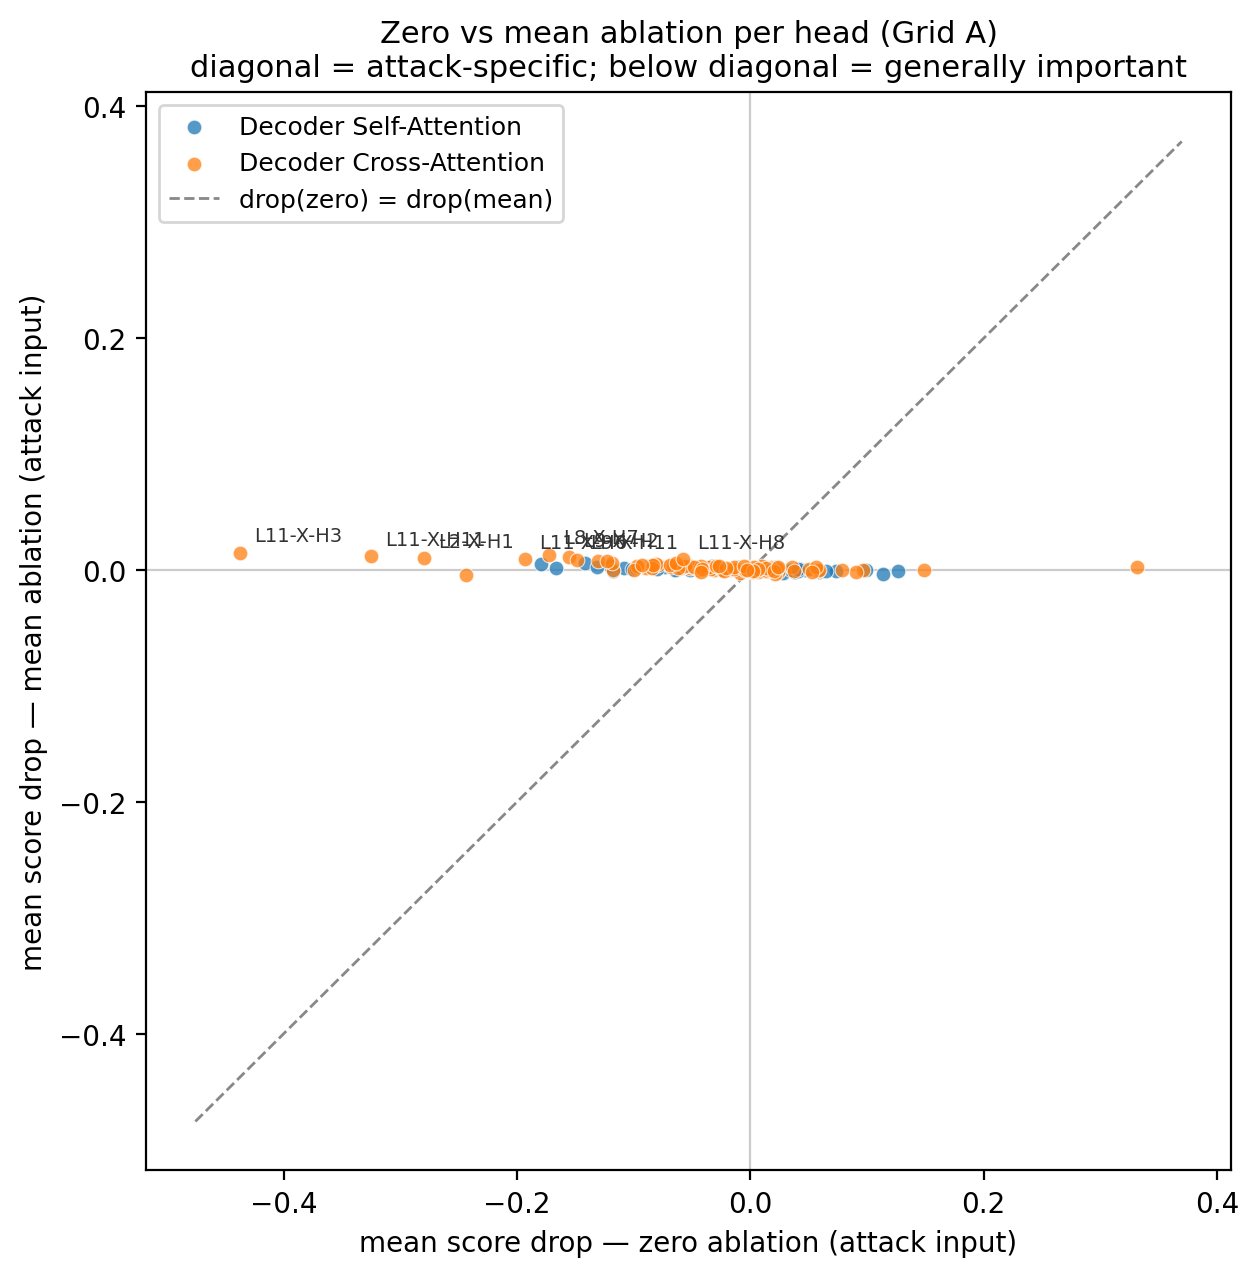
\includegraphics[width=0.95\textwidth]{outputs/plots/zero_vs_mean_ablation_scatter.png}
  \caption{Mean score drop from zero ablation (x-axis) vs. mean ablation
  (y-axis), per head, Grid~A. The important heads sit far from the
  drop(zero)=drop(mean) diagonal: large negative zero-ablation drop,
  small positive mean-ablation drop.}
  \label{fig:scatter}
\end{figure}

\begin{figure}[H]
  \centering
  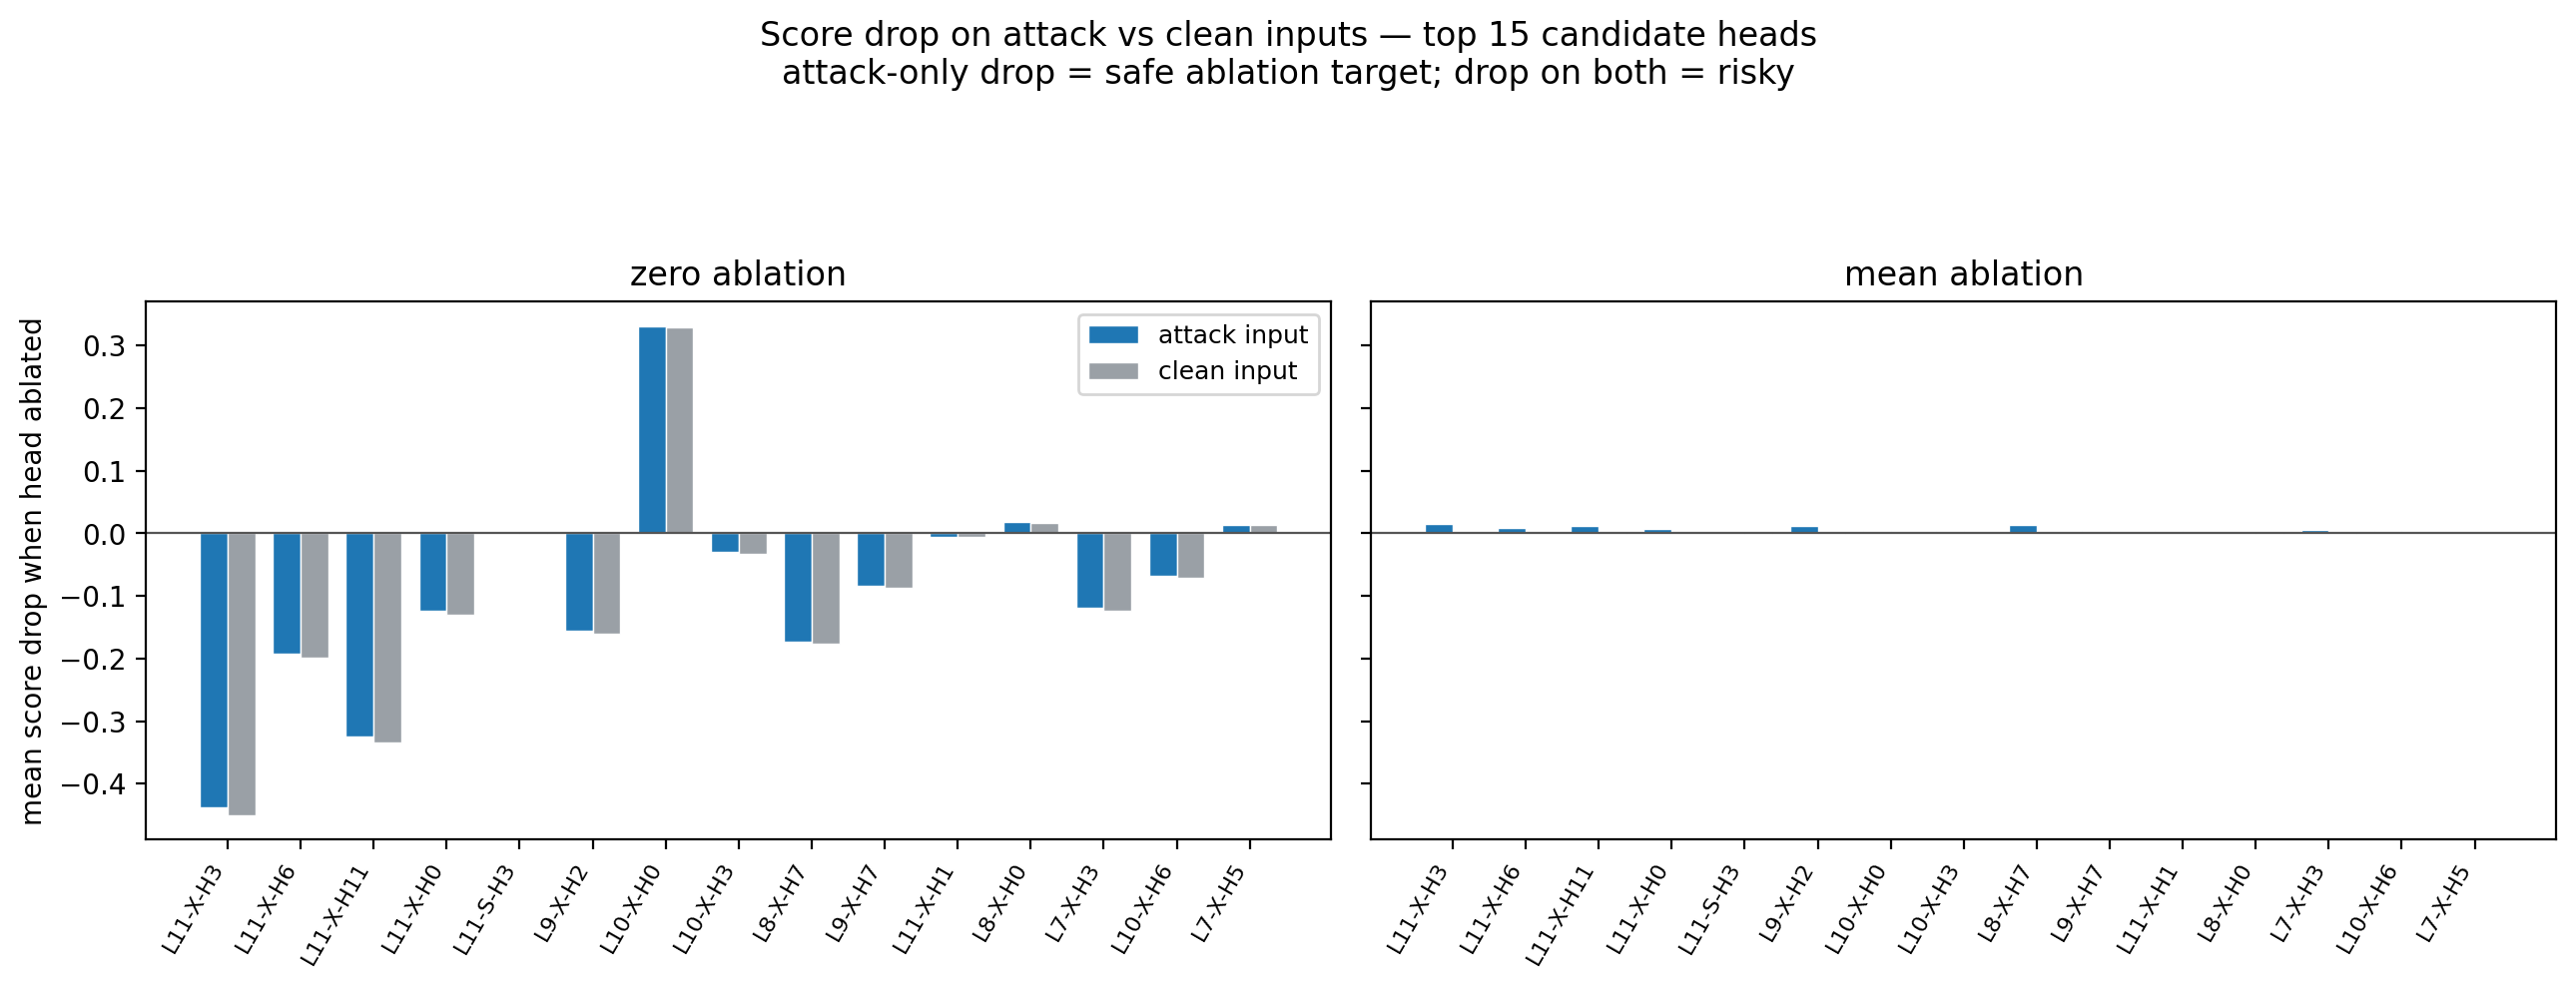
\includegraphics[width=0.95\textwidth]{outputs/plots/clean_vs_attack_drop.png}
  \caption{Mean score drop when ablating each of the top 15 candidate
  heads, on the attack input (Grid~A) vs. the matched clean input
  (Clean~A). Left: zero ablation. Right: mean ablation.}
  \label{fig:barchart}
\end{figure}

Figures~\ref{fig:scatter}--\ref{fig:barchart} reveal a finding that would be
invisible from the localisation heatmap alone. For the top candidate heads
(e.g.\ \texttt{L11-X-H3}):
\begin{itemize}[nosep]
  \item \textbf{Zero ablation} causes a large score change on the attack
  input ($\text{drop}_{\text{zero}}=-0.437$, i.e.\ the score \emph{rises}
  when the head is zeroed) that is \emph{nearly identical} on the clean
  input ($-0.450$). Zeroing this head is a generic, out-of-distribution
  perturbation that disturbs the model's scoring behaviour regardless of
  whether the input is attacked — a large but \textbf{non-attack-specific}
  effect, and thus a \emph{risky} ablation target if the goal is a targeted
  defence.
  \item \textbf{Mean ablation} — substituting the head's own
  padded-control activation, a distribution-matched value rather than an
  artificial zero — causes a much smaller drop on the attack input
  ($+0.015$) and essentially \emph{no} drop on the clean input
  ($+0.0001$). This is small in magnitude but genuinely
  \textbf{attack-specific}: exactly the signature Experiment~1's
  reverse-patching methodology was designed to isolate.
\end{itemize}
The same pattern holds for all top-5 heads (Table~\ref{tab:top8}):
zero-ablation drops are large and essentially clean-vs-attack-indistinguishable,
while mean-ablation drops are an order of magnitude smaller but consistently
attack-only. The practical implication is that \textbf{zero ablation, taken
alone, over-states and mis-attributes head importance}: it conflates ``this
head does something the model needs in general'' with ``this head carries
the attack signal''. Mean ablation (equivalently, reverse patching) is the
more reliable diagnostic for attack-specific attribution, while zero
ablation is better read as a measure of the head's general functional
necessity. This pattern is unchanged between $n=10$ and $n=100$ — unlike
head universality and Grid~A/B agreement, the zero-vs-mean asymmetry is not
an artefact of sample size.

\subsection{What changed from $n=10$ to $n=100$, and why}
\label{sec:n100}

Grid~A and Clean~A were originally run at 10 examples/attack; this section
documents, explicitly, what the ten-fold increase in sample size changed
and why — both because transparency about revised findings matters, and
because Experiments~6 and 7 (which build on this experiment's flagged-head
list) may have been launched against whichever head-summary snapshot
existed at the time they ran, so this record clarifies which numbers were
current when.

\paragraph{More heads clear the significance threshold — expected, not
alarming.} 13/288 at $n=10$ became 33/288 at $n=100$. A fixed threshold
against a mean estimated from fewer examples is under-powered: some heads
with a real but modest effect simply did not accumulate enough signal at
$n=10$ to clear $0.02$. This is the ordinary behaviour of averaging over
more data, not a sign the $n=10$ run was wrong within its own precision.

\paragraph{Head universality was overstated at $n=10$.}
\texttt{L11-X-H3}'s reported range at $n=10$, $[0.027, 0.102]$, undersold
both its true ceiling (attacks exist where its effect reaches $0.72$) and
its true floor (one attack, \texttt{bar\_random\_4}, is actually negative).
Ten examples per attack is enough to estimate a \emph{mean} well but not
enough to see the tails of the per-attack distribution — the claim
``positive on all 105 attacks'' should have been read as ``positive on all
105 attacks \emph{in this sample}'', and the $n=100$ run shows that caveat
was load-bearing.

\paragraph{Grid~A/B agreement was overstated at $n=10$ — this is the most
consequential revision.} The correlation between breadth (Grid~A) and depth
(Grid~B) dropped from $r=0.84$ to $r=0.42$ once both grids had equal
statistical power. Inspecting the individual heads responsible clarifies
why: \texttt{L1-X-H7} shows the single largest Grid~A/B gap
($-0.107$ vs.\ $+0.023$), and its Grid~A mean is dominated by one
attack with an extreme value ($-2.95$ on some attack, pulling the mean far
below the median of $-0.012$) — a heavy-tailed, outlier-driven head, not a
stably important or unimportant one. More broadly, only 7 of Grid~A's 33
significant heads are \emph{also} significant in Grid~B, meaning most
heads flagged by the 105-attack breadth sweep are specific to attacks
\emph{other than} the canonical \texttt{relevant\_start\_5} — attack
specificity is more pervasive than the $n=10$ pilot suggested, not less.
Practically: a flagged-head list intended to generalise across attacks
should be read from Grid~A (breadth), not Grid~B (one attack's depth), and
even Grid~A's list should be treated as noisier and more attack-contingent
than the original report implied.

\paragraph{What did \emph{not} change.} The core mechanistic claims are
robust to sample size: cross-attention dominates self-attention (now even
more starkly — self-attention's mean effect is statistically
indistinguishable from zero, not just small); forward and reverse patching
agree almost exactly for every head; and zero ablation is large-but-generic
while mean ablation is small-but-attack-specific. These are the findings
this report's abstract and discussion should be read as resting on.

% =====================================================================
\section{Overall Interpretation and Discussion}
% =====================================================================

\begin{enumerate}
  \item \textbf{The layer-level signal is carried by a small, specific set
  of cross-attention heads, not spread evenly.} 33/288 head-slots (11.5\%)
  matter appreciably, and self-attention's mean effect is statistically
  indistinguishable from zero. This sharpens Experiment~1's ``late decoder
  cross-attention'' finding into a short, falsifiable (if larger than
  initially estimated) list of specific heads.
  \item \textbf{Two distinct causal roles coexist within the top heads.}
  \texttt{L11-X-H3} is a \emph{near-universal} carrier (positive on 104 of
  105 attacks); \texttt{L9-X-H2} is a \emph{specialist} that dominates on
  particular attacks (peaking on \texttt{true\_end\_4}, not even the
  canonical \texttt{relevant\_start\_5}) but is silent or mildly harmful on
  roughly a quarter of attacks. A single ranker defence would need to
  address both types.
  \item \textbf{Forward and reverse patching agree almost exactly}
  (mean $|\fwd-\rev|=0.00034$) — the important heads are cleanly both
  sufficient and necessary, with no evidence of compensation or
  redundancy among them. Unchanged between $n=10$ and $n=100$.
  \item \textbf{Ablation-method choice materially changes the conclusion.}
  Zero ablation makes every top head look catastrophically important and
  gives no way to distinguish ``breaks the attack'' from ``breaks
  everything''; mean ablation isolates the attack-specific component
  cleanly, at the cost of a much smaller absolute signal. Any future
  head-ablation defence should be evaluated with mean (distribution-matched)
  ablation, not zero ablation, to avoid mistaking general functional
  importance for attack-specific involvement. Also unchanged between $n=10$
  and $n=100$.
  \item \textbf{Grid~A and Grid~B cross-validate only weakly at full
  statistical power.} At $n=10$ the two grids appeared to agree strongly
  ($r=0.84$); at $n=100$ for both, $r$ drops to $0.42$, and only 7 of
  Grid~A's 33 significant heads are also significant in Grid~B. This
  revises, rather than confirms, the original conclusion: breadth
  (Grid~A) and single-attack depth (Grid~B) genuinely disagree on
  \emph{which} heads matter, because most heads are more attack-specific
  than a single canonical example can reveal. A downstream consumer of
  this experiment's ``flagged heads'' (e.g.\ Experiment~7's per-head logit
  lens) should treat the list as breadth-representative but noisy, not as
  a small set of universally important heads.
\end{enumerate}

% =====================================================================
\section{Limitations and Threats to Validity}
% =====================================================================

\begin{itemize}
  \item \textbf{Decoder-only, two components.} The encoder and the decoder
  feed-forward network are out of scope; Experiment~1 suggests the encoder
  self-attention pathway (for the multi-step generation case) or the
  decoder MLP could carry residual signal not visible here.
  \item \textbf{Single decoder step.} All activations are $(1,1,768)$
  because monoT5 scoring never generates beyond the first token. The
  batched-over-heads and encoder-reuse speedups both depend on this and
  would not directly carry over to a generative scoring setup.
  \item \textbf{Sample size.} Grid~A now matches Grid~B's depth (100
  examples/attack, up from an initial 10/attack pilot), which is precisely
  what exposed the weak Grid~A/B correlation (Section~\ref{sec:n100}) — the
  two do \emph{not} agree well at matched statistical power, which is
  itself evidence that per-attack sample size, not just total attack count,
  materially affects these conclusions. A further increase (e.g.\ 200/attack
  where available) was not run; whether $r=0.42$ is itself still
  under-converged is open.
  \item \textbf{No joint/multi-head ablation.} This experiment only ablates
  one head at a time. Whether the top 33 heads act redundantly (ablating
  all of them together removes little more than the best single head) or
  additively (each contributes independently) is left for future work, as
  specified in the experiment scope.
  \item \textbf{Single model / dataset.} Results are for monoT5-base
  (12 layers, 12 heads, $d_{kv}=64$) on DL19, matching Experiment~1's setup.
\end{itemize}

% =====================================================================
\section{Reproducibility}
% =====================================================================

From \texttt{03\_monot5\_head\_patching\_ablation/}, with the
\texttt{advseq2seq} conda environment (same dependencies as
Experiment~1) and Experiment~1's outputs already present as a sibling
directory (\texttt{../01\_monot5\_layer\_patching/outputs/attacks/}):

\begin{lstlisting}
bash bash/run_tests.sh          # unit tests (tiny random T5, CPU)
bash bash/run_smoke.sh          # end-to-end smoke test -> outputs_smoke/
bash bash/run_all.sh            # full pipeline (resume-safe)

# or stage-by-stage:
python scripts/01_run_head_grid.py --config configs/default.yaml --run all
python scripts/02_aggregate.py   --config configs/default.yaml
python scripts/03_make_plots.py  --config configs/default.yaml
\end{lstlisting}

\noindent Initial pilot (Grid~A/Clean~A at $n=10$): SLURM job on
1$\times$ L40 GPU, $\approx$38 minutes wall-clock for all four runs plus
aggregation and plotting. Revised run (Grid~A/Clean~A re-run at $n=100$
via \texttt{scripts/01\_run\_head\_grid.py --run grid\_a --force} and
\texttt{--run clean\_a --force}, then re-aggregated): $\approx$4 hours
wall-clock. Outputs under
\texttt{outputs/\{grid\_a,grid\_b,clean\_a,clean\_b\}/} and
\texttt{outputs/plots/} reflect the $n=100$ revision throughout.

% =====================================================================
\section*{Appendix: Glossary of Key Quantities}
\addcontentsline{toc}{section}{Appendix: Glossary of Key Quantities}
% =====================================================================

\begin{description}[leftmargin=1.6em,style=nextline]
  \item[$\score$] $\operatorname{logit}(\texttt{true})-\operatorname{logit}(\texttt{false})$ at the single decoder step.
  \item[head-slot] one (decoder layer, component, head index) triple; 288 total.
  \item[$\fwd_{L,C,h}$ / $\rev_{L,C,h}$] forward/reverse patching effect of head $h$, Eqs.~\ref{eq:hfwd}--\ref{eq:hrev}.
  \item[$\comb_{L,C,h}$] $\min(\fwd,\rev)$ — both sufficient and necessary, Eq.~\ref{eq:hcomb}.
  \item[zero ablation] head output forced to the zero vector.
  \item[mean ablation] head output replaced by its padded-control (Type~B) activation; algebraically equal to reverse patching on the attack base.
  \item[score\_drop] $\score_{\text{before}} - \score_{\text{ablated}}$, Eq.~\ref{eq:drop}.
  \item[Grid A / B] breadth (105 attacks, $n{=}100$) / depth (1 attack, $n{=}100$) patching+ablation runs on attack inputs; Grid~A was originally piloted at $n{=}10$ (Section~\ref{sec:n100}).
  \item[Clean A / B] the same two example sets, ablation-only, scored on the unattacked clean input (side-effect check).
  \item[near-universal head] positive combined effect on nearly all 105 attacks (104/105 for the top head), e.g.\ \texttt{L11-X-H3}.
  \item[attack-specific head] high combined effect on a subset of attacks, near-zero or negative on others, e.g.\ \texttt{L9-X-H2}.
\end{description}

\end{document}
